\documentclass{scrartcl}

\usepackage[utf8]{inputenc}
\usepackage[T1]{fontenc}
\usepackage{lmodern}
\usepackage[english]{babel}
\usepackage{amsmath}
\usepackage{graphicx}
\usepackage{caption}	
\usepackage{subcaption}	 
\usepackage{hyperref}
\usepackage[parfill]{parskip}
\usepackage{hhline}

\title{Neuroprosthetics - Exercise 1}
\author{Alexander Koenig}
\date{16. November 2019}

\begin{document}
\maketitle

\section{Signal Generation}

A superposition of signals can be calculated with equation \ref{eq:signal} where $A_{o}$ is the signal offset, and $A_{i}$ is the amplitude of the frequency component $F_{i}$. 
\begin{equation}
	\label{eq:signal}
	f(t) = A_{o} + \sum_{i=1}^{n}A_{i} \cdot\sin (2\pi F_{i} \cdot t)
\end{equation}

Figure \ref{fig:signal} shows the superposition of three signals with the below properties and an offset $A_{o}$ of 3. The signal was created with equation \ref{eq:signal} and a sampling rate of 100kHz. 

\begin{table}[h]
\centering
\begin{tabular}{|l|l|l|}
\hline
$i$ & $A_{i}$ & $F_{i}$ \\ \hhline{|=|=|=|}
1   & 1       & 100 Hz  \\ \hline
2   & 1.5     & 600 Hz  \\ \hline
3   & 2       & 9 kHz   \\ \hline
\end{tabular}

\label{tab:values}
\end{table}
\begin{figure}[h]
	\centering
	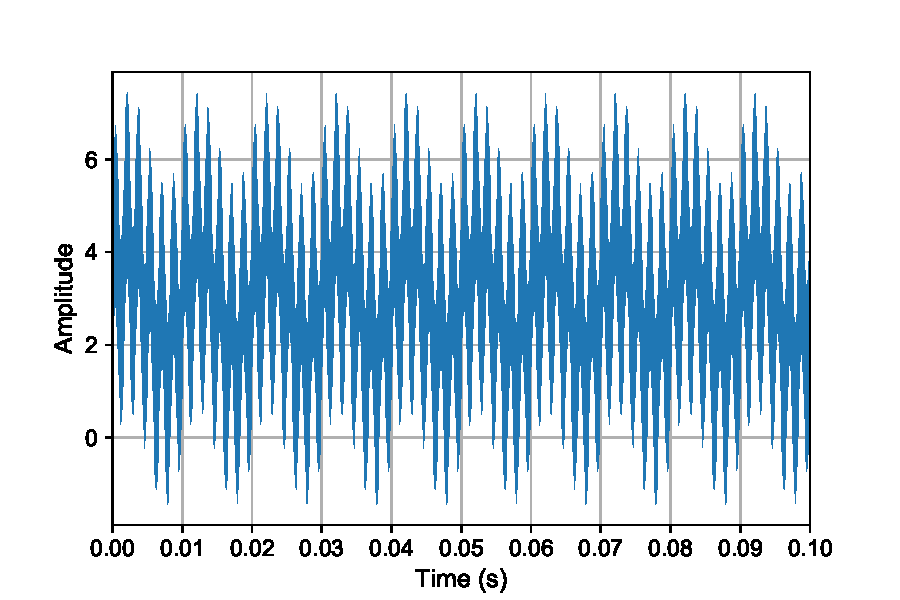
\includegraphics[width=0.95\textwidth]{figures/signal.pdf}
	\caption{First 100ms of superimposed signal}
	\label{fig:signal}
\end{figure}

\section{Single Sided Spectrum}

Figure \ref{fig:spectra} shows the reconstructed single-sided amplitude spectra of the previously presented superimposed signal with different sample rates. The single-sided spectra were calculated by using NumPy's implementation of the Fast Fourier Transformation (FFT). It becomes clear that for a sample rate of 100kHz and 20kHz the underlying frequencies of the signal can be correctly reconstructed. However, this is not the case for the sampling rate of 10kHz as a frequency bin at 1kHz can be observed although it does not correspond to a base frequency.

In signal processing, this phenomenon is called aliasing. Aliasing effects occur if the analyzed signal contains frequencies that are higher than half of the sampling rate. Mathematically, this is expressed by the Nyquist-Shannon sampling theorem (equation \ref{eq:nyquist-shannon}). The corresponding threshold is called the Nyquist frequency (equation \ref{eq:nyquist}).

\begin{equation}
	\label{eq:nyquist}
	f_{nyquist} = \frac{1}{2}\cdot f_{sampling}
\end{equation}
\begin{equation}
	\label{eq:nyquist-shannon}
	f_{signal} < f_{nyquist}
\end{equation}

In the described case the Nyquist frequency is $f_{nyquist} = \frac{1}{2}\cdot 10$kHz $= 5$kHz. This in turn means that to fully reconstruct the signal it must not contain any frequencies greater or equal to 5kHz. However, since the base frequency $F_{3} = 9$kHz is greater than the Nyquist frequency, the signal cannot be correctly reconstructed and aliasing effects occur. To prevent aliasing a low-pass filter can be applied to the signal before the calculation of the spectrum.

\begin{figure}[p]
	\centering
	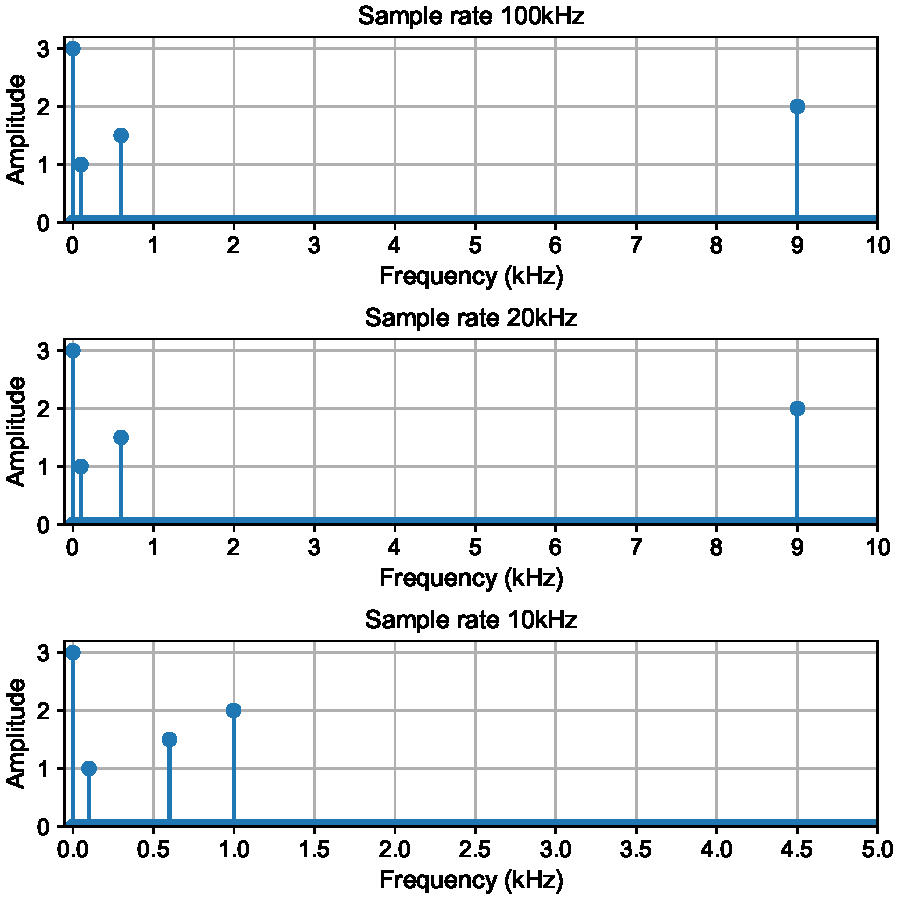
\includegraphics[width=0.9\textwidth]{figures/spectra.pdf}
	\caption{Single sided amplitude spectra for different sample rates}
	\label{fig:spectra}
\end{figure}
\end{document}